\section{Forberedelse før test}\label{afs:tests}
Før testene kan gå i gang, skal en testplan udarbejdes således begge versioner bliver testet under samme vilkår med samme funktionaliteter. En tabel over testene kan ses i tabel \ref{tab:resultat_diskret}.
\\

Til test af begge versioner konstrueres en batteriholder til de fire celler som ses på figur \ref{fig:battery_holder}. Her er en ledning forbundet til hver celle for balancering af spændingsmåling.

\begin{figure}[h]
	\centering
	\includegraphics[width=11cm]{billeder/battery_holder.jpg}
	\caption{Batteriholder med balanceringsstik.}
	\label{fig:battery_holder}
\end{figure}

\section{Test af IC version}\label{afs:test_ic}
I dette afsnit vil en komplet test opstilling af den integrerede version af BMS'en blive gennemgået og udført. Alle implementerede funktionaliteter beskrevet i kapitel \ref{kap:funktionaliteter} testes for ønsket og optimal funktion. 

\subsection{Testopstilling}
Ved brug af en elektrisk belastning (til venstre på figur \ref{fig:ic_testsetup}) vil den maksimale afladestrøm blive testet. Der bruges en laboratoriestrømforsyning (midten til højre) til test af opladefunktionalitet. Et oscilloskop med $1^2C$ protokol dekodning bruges til aflæsning af registre og adressering (midten til venstre) og til sidst en computer med et terminal program til brugergrænsefladen (shell). 

\begin{figure}[h]
	\centering
	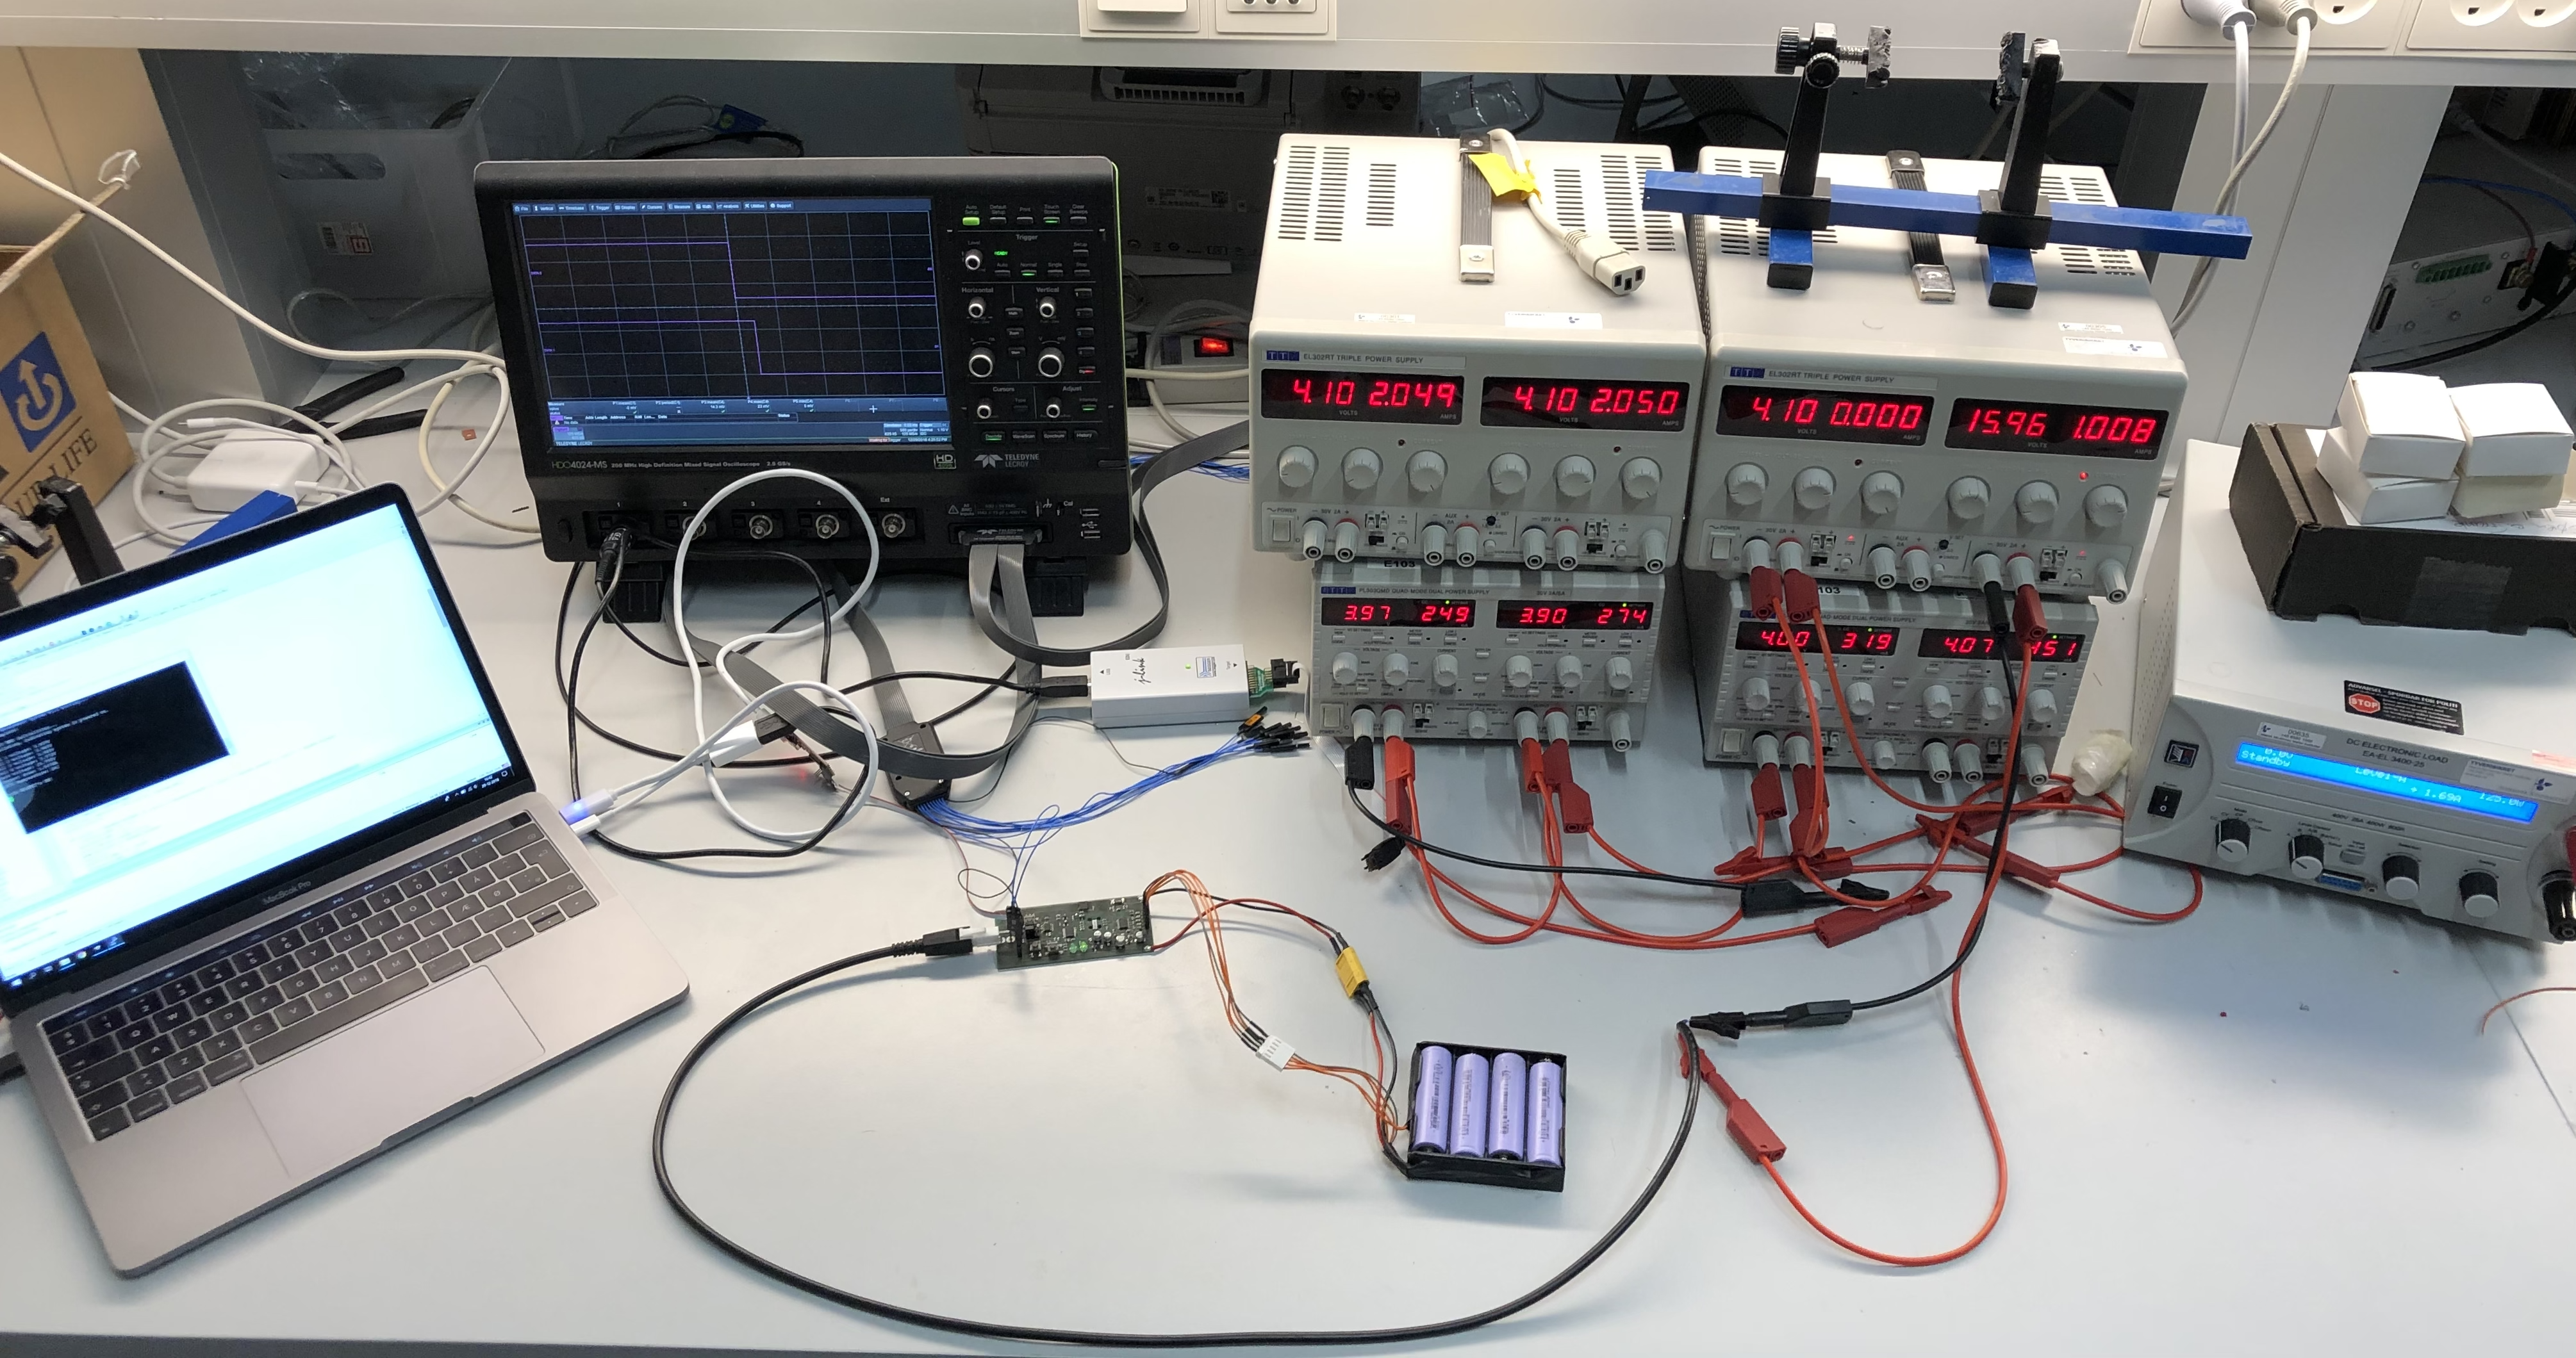
\includegraphics[width=15cm]{billeder/integreret_testsetup.png}
	\caption{Testopsætning til IC versionen}
	\label{fig:ic_testsetup}
\end{figure}

\subsection{Resultat skema}
Resultaterne fra testene kan ses i tabel \ref{tab:resultat_IC}.

\begin{table}[h!]
	\small
	\centering
	\begin{threeparttable}
		\begin{tabular}{ l l l l l l l }
			\toprule
			\multicolumn{1}{l}{\textbf{Funktionalitet}}          &
			\multicolumn{1}{l}{\textbf{Resultat}}           \\
			\hline
			Spændingsmålinger              & Virker                         \\
			Afladestrømmåling                    		& Virker                         \\
			Opladestrømmåling                    		& Virker ikke optimalt                         \\
			Temperaturmåling                    		& Virker                       \\
			Afladestrømsbeskyttelse		& Slår fra ved $6\ampere$        \\
			Opladestrømsbeskyttelse   	& Slår ikke fra da målingen ikke virker optimalt      \\
			Temperaturbeskyttelse          & BMS afbryder ved $\SI{45}{\celsius}$ og venter indtil nedkølet til $\SI{40}{\celsius}$           \\
			Balancering af celle 1         & Virker                         \\
			Balancering af celle 2        & Virker                         \\
			Balancering af celle 3        & Virker                         \\			
			Balancering af celle 4        & Virker                         \\
			Balancering færdig             & BMS afbryder og informerer brugeren                  \\
			Information om kapacitet       & Virker                          \\
			Information om batteriprocent 							& Virker			 \\
			Brugergrænseflade (Shell)                       & Virker                    \\
			%    &      &       \\
			
			\bottomrule
		\end{tabular}
		%\begin{tablenotes}
		%	\item[a] \textit{Kommentar}
		%\end{tablenotes}
		\caption{Resultatliste over test af integreret version.}
		\label{tab:resultat_IC}
	\end{threeparttable}
\end{table} 
\FloatBlock

\subsection{Delkonklusion}
Som der ses i tabellen \ref{tab:resultat_IC} virker de fleste af funktionerne. Opladestrømmålingen fejler da der sker en fejl i konverteringen af 16-bit 2's complement tallet, og derfor returnerer et mærkeligt tal, og er årsagen til at opladebeskyttelsen ikke virker. Denne fejl er ikke rettet da det ikke ville være hensigtsmæssigt med hensyn til tiden. Dog er det også under afladning at beskyttelsen er mest vigtig, da der oftest kortsluttes/aflades for hårdt, end at en for kraftig oplader tilsluttes.

\section{Test af diskret version}\label{afs:test_diskret}
I dette afsnit vil en komplet test opstilling af den diskrete version af BMS'en blive gennemgået og udført. Alle implementerede funktionaliteter beskrevet i kapitel \ref{kap:funktionaliteter} testes for ønsket og optimal funktion. 

\subsection{Testopstilling}
Da microcontrolleren ikke kunne monteres og derfor ikke kunne testes på denne version, blev testopstillingen lidt anderledes. Her bruges en laboratoriestrømforsyning (til venstre på figur \ref{fig:diskret_testsetup}) til at sætte de spændinger som microcontrolleren skulle gøre ved hjælp af PWM på henholdsvis $1,7\volt$ til afladefetten og $300\milli\volt$ til opladefetten. Derudover er der en strømforsyning til test af opladning (midten, øverst), og en elektrisk belastning til test af afladning (midten, nederst). Balanceringen er testet manuelt ved hvert enkelt ben. Oscilloskopet (til højre) bruges til aflæsning af værdierne på strømmålings-operationsforstærkernes indgangsben.

\begin{figure}[h]
	\centering
	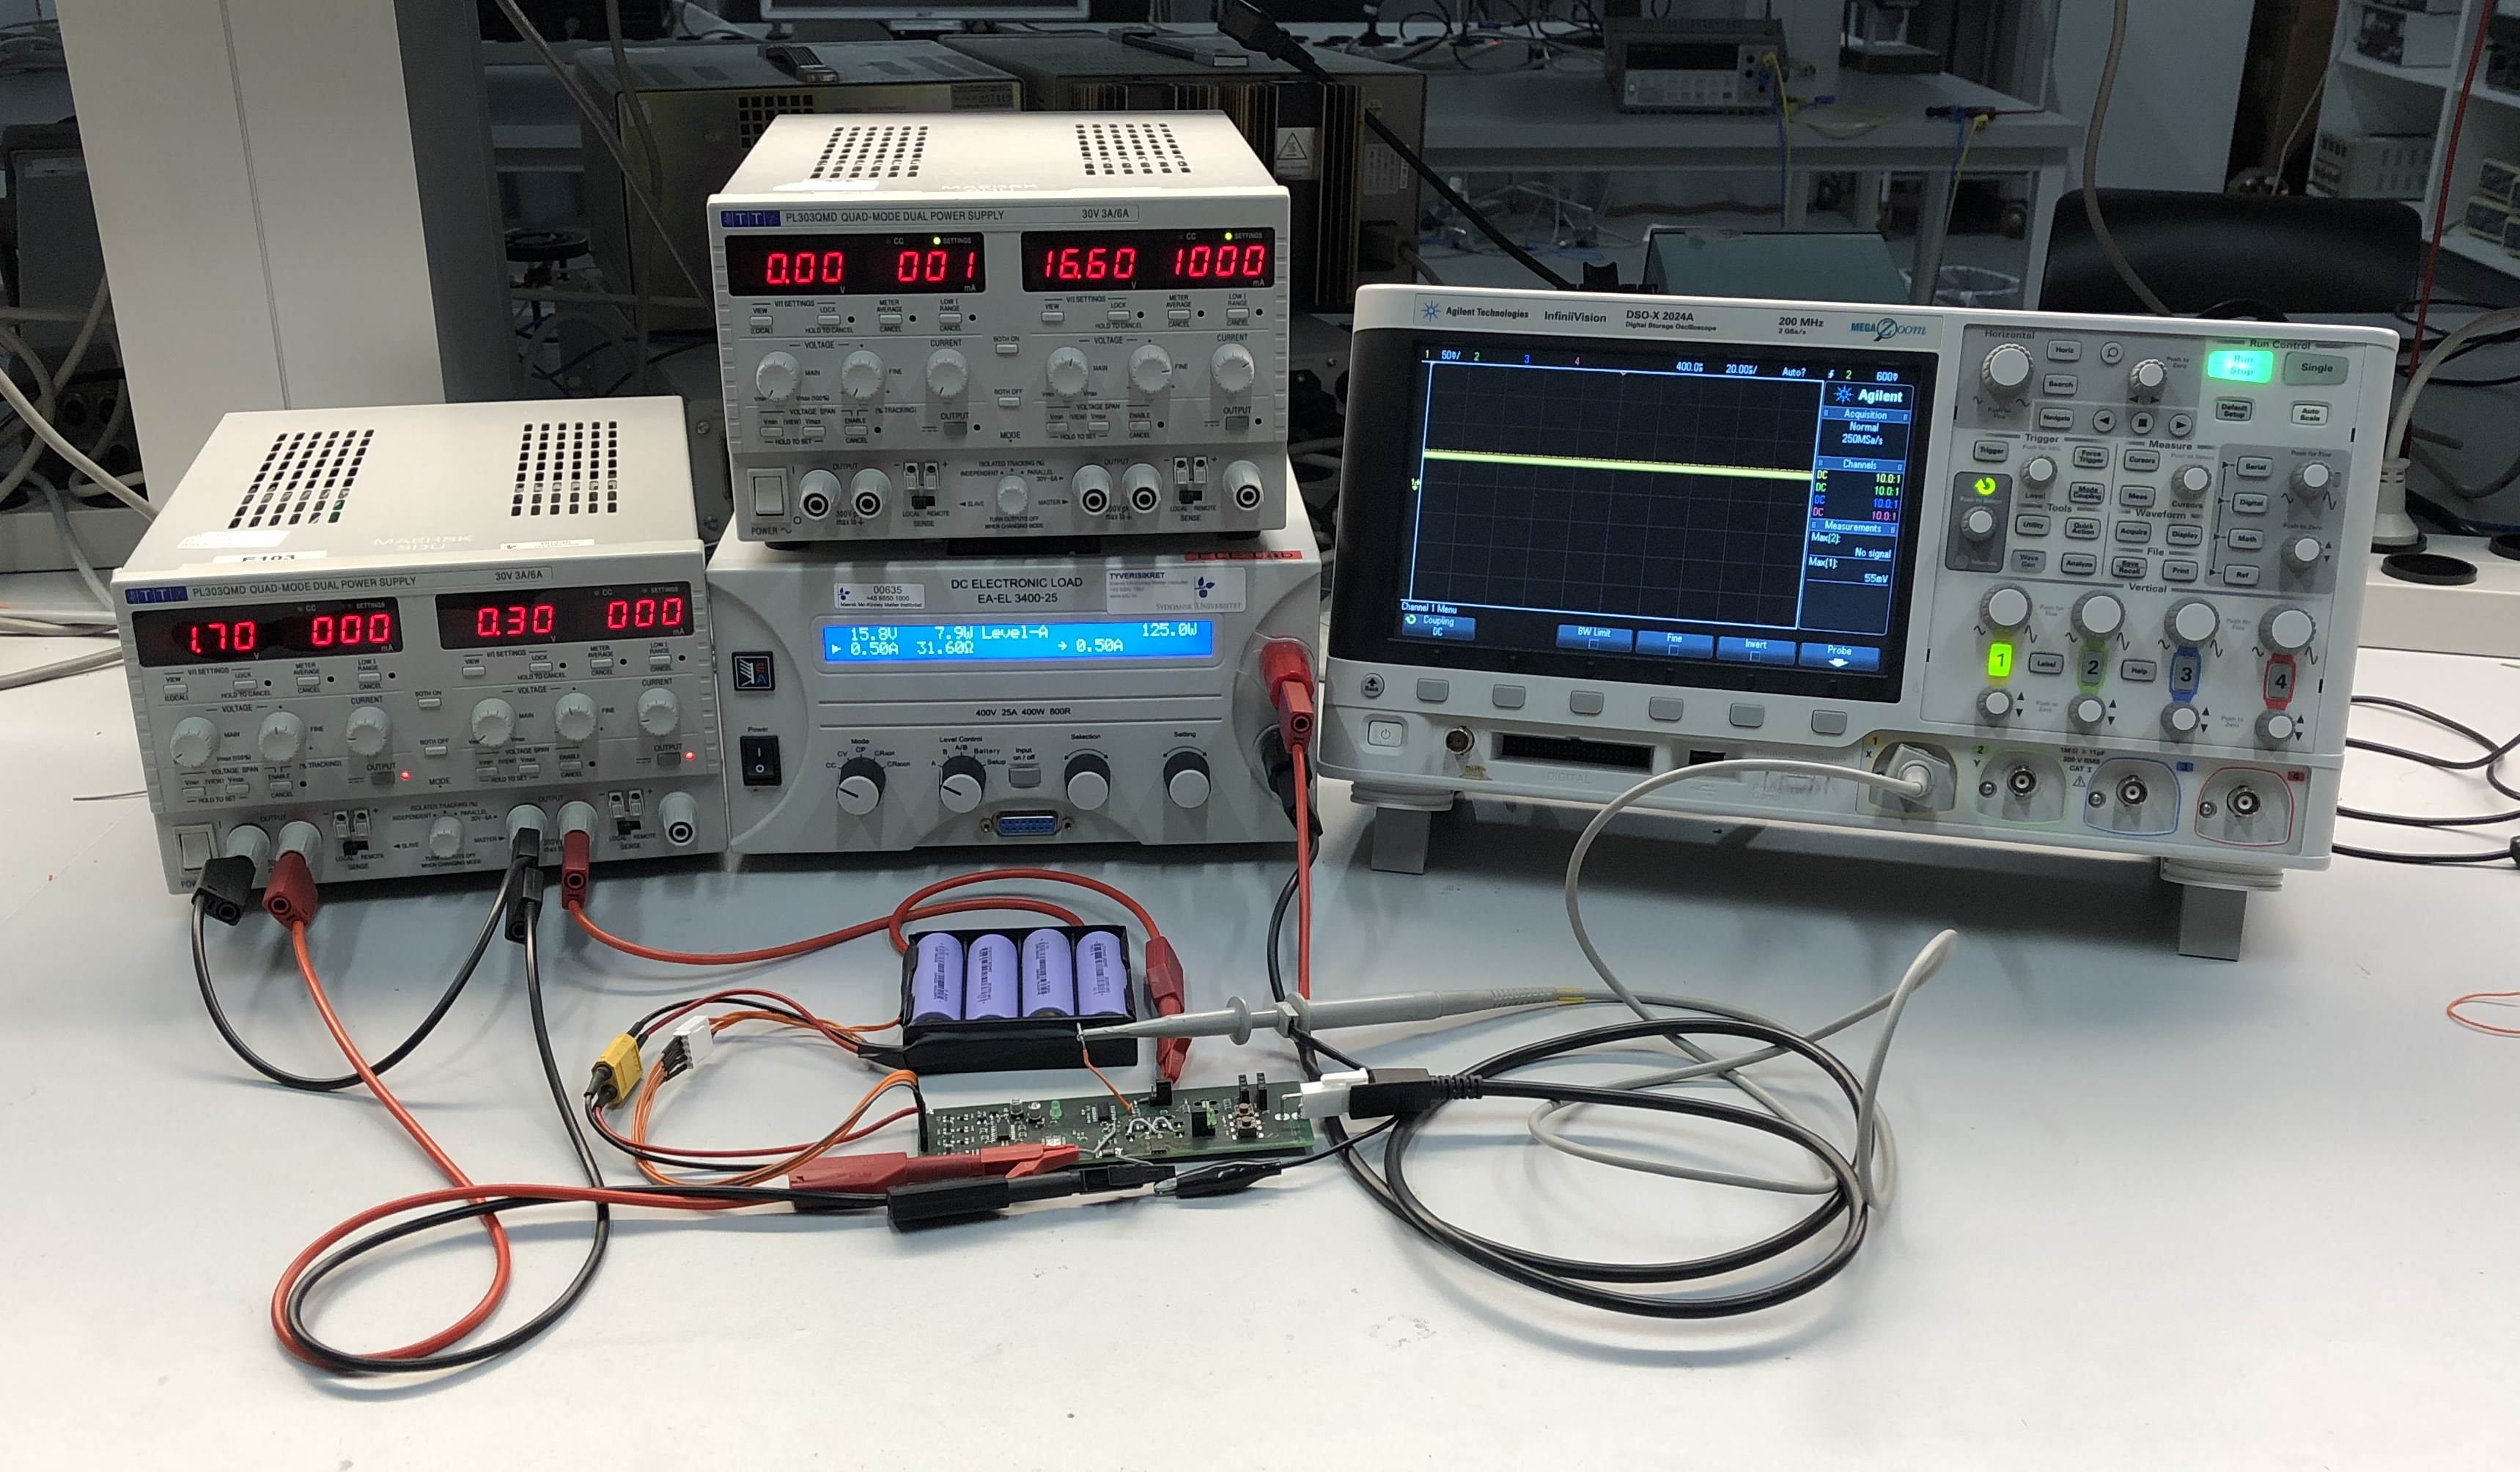
\includegraphics[width=15cm]{billeder/diskret_testsetup.png}
	\caption{Testopsætning til den diskrete version}
	\label{fig:diskret_testsetup}
\end{figure}

\subsection{Resultat skema}
Resultaterne fra testene kan ses i tabel \ref{tab:resultat_diskret}.

\begin{table}[h!]
	\small
	\centering
	\begin{threeparttable}
		\begin{tabular}{ l l l l l l l }
			\toprule
			\multicolumn{1}{l}{\textbf{Funktionalitet}}          &
			\multicolumn{1}{l}{\textbf{Resultat}}           \\
			\hline
			Spændingsmålinger              & Virker                         \\
			Afladestrømmåling                    		& Virker                         \\
			Opladestrømmåling                    		& Virker                         \\
			Temperaturmåling                    		& Kan ikke testes, men er det samme som IC versionen    \\
			Afladestrømsbeskyttelse		& Slår fra ved $4.3\ampere$        \\
			Opladestrømsbeskyttelse   	& Slår fra ved $0.6\ampere$      \\
			Temperaturbeskyttelse          & Kan ikke testes, men er det samme som IC versionen          \\
			Balancering af celle 1         & Virker manuelt                         \\
			Balancering af celle 2        & Virker manuelt                        \\
			Balancering af celle 3        & Virker manuelt                        \\			
			Balancering af celle 4        & Virker manuelt                        \\
			Balancering færdig             & Stopper ikke, da der ikke er nogen microcontroller til kontrol.               \\
			Information om kapacitet       & Ikke muligt                          \\
			Information om batteriprocent 							& Ikke muligt			 \\
			Brugergrænseflade (Shell)                       & Ikke muligt                    \\
			%    &      &       \\
			
			\bottomrule
		\end{tabular}
		%\begin{tablenotes}
		%	\item[a] \textit{Kommentar}
		%\end{tablenotes}
		\caption{Resultatliste over test af diskret version.}
		\label{tab:resultat_diskret}
	\end{threeparttable}
\end{table} 
\FloatBlock

\subsection{Delkonklusion}
Ud fra test af denne version kan der konkluderes at, på trods af manglende microcontroller, kunne de vigtigste funktionaliteter stadig testes manuelt. Den maksimale op- og ladeladestrøm slog fra før den skulle. Derfor blev tests foretaget med at forøge reference spændingen på op- og afladebenet, hvortil den ønskede cut-off strøm kunne opnås. Der blev i projektet ikke fundet ud af, hvorfor strømmene blev afbrudt før målet.
\\

For at test balancering af cellerne, blev MOSFET'erne manuelt slukket grundet manglende styring fra microcontrolleren. Derefter kunne balancering testes ved at holde opladte cellers ben højt og trække spændingen lav på celler under balancering.





